\documentclass[screen]{beamer}
\usepackage[T1]{fontenc}
\usepackage[utf8]{inputenc}
\usepackage{multimedia}
\usepackage{subcaption}
\usepackage{algorithm}
\usepackage{algorithmic}
\usepackage{bm}


% Bruk NTNU-temaet for beamer (her i bokmålvariant), alternativer er
% ntnunynorsk og ntnuenglish.
\usetheme{ntnuenglish}
 
% Angi tittelen, vi gir også en kortere variant som brukes nederst på
% hver slide:
\title[Eksempelforedrag]%
{COOL AND AWESOME TITLE}

% Denne kan du også bruke hvis det passer seg:
%\subtitle{Valgfri undertittel}

% Angir foredragsholder, også en (valgfri) kortversjon i
% hakeparanteser først som kommer nederst på hver slide:
\author[aut]{Aga, Kristian \\ Berge, Runar L. \\ Klemetsdal Øystein S.,\\
	Myrvoll-Nilsen, Eirik \\ Selle, Maria.
}


% Institusjon. Bruk gjerne disse slik det passer best med det du vil
% ha.  Valgfri kortversjon her også
%\institute[NTNU]{Institutt for matematiske fag}

% Datoen blir også trykket på forsida. 
\date{November 23., 2015}
%\date{} % Bruk denne hvis du ikke vil ha noe dato på forsida.

% Fra her av begynner selve dokumentet
\begin{document}

% Siden NTNU-malen har en annen bakgrunn på forsida, må dette gjøres
% i en egen kommando, ikke på vanlig beamer-måte:
\ntnutitlepage

\begin{frame}{Generation of wave}
	\begin{itemize}
		\item %Assumptions about stone; 
		One big cohesive stone, uniform qaudratic shape in horizontal plane.
		\item Terminal Speed in water
	\end{itemize}
	\begin{align*}
		F_g=F_b+D\\
		%F_g=V\rho_{R}g\\
		%F_b= V \rho_{w}g\\
		%D=\frac{1}{2}C_d\rho_{w}Av^2 C_d\\
		v_{\infty}=\sqrt{\frac{2Vg(\rho_R-\rho_W)}{C_d A \rho_W}} \approx 145 m/s
	\end{align*}
	\begin{itemize}
		\item Drop from mountainside to the surface (phase 1).\\
		Drop from the surface of the fjord to the bottom (phase 2).
	\end{itemize}
	
\end{frame}


\begin{frame}{Generation of wave}
	Speed as wave reaches the water ($mah = \frac{1}{2}mv^2$)
	\begin{itemize}
		\item Free fall $\rightarrow v_{upper}=54$m/s.
		\item Inclined plane $\theta=45^{\circ}$ and $\gamma = 0.6$ $\rightarrow a=g(\sin(\theta) - \gamma cos(\theta)) \rightarrow v_{lower}=35$ m/s\\
	\end{itemize}
	\pause
	Energy converted to wave
	\begin{itemize}
		\item Surface tension, shape of rock, impact
		\item Upper estimate 50\% $\rightarrow E_{upper} =\frac{1}{2}m v_{upper}^2 \cdot 50\% = 9.8\cdot10^{13}$ J
		\item Lower estimate 1\% $\rightarrow E_{lower} =\frac{1}{2}m v_{lower}^2 \cdot 1\% = 7.8 \cdot 10^{11}$ J
	\end{itemize}
	
\end{frame}


\begin{frame}{Analysis of linear equations}
	\begin{block}{PDE}
	\begin{equation*}
		\begin{cases}
				\mu \phi _{xx} + \phi_{zz} = 0&\\
		\phi _z = 0	, &	 				\quad	z = -1	\\
			\mu \phi_{tt} + \phi_z = 0	, & \quad z = 0.
		\end{cases}
	\end{equation*}
	\end{block}
	\pause
	\begin{equation*}
		\phi(x,z,t) = X(x)Z(z)T(t),\quad 		\mu\frac{X''(x)}{X(x)} = - \frac{Z''(z)}{Z(z)} = k
	\end{equation*}

	\begin{equation*}
		\phi(x,z,t) = \sum_{n=0}^{\infty}  Z_n(z)e^{i\left(\frac{\pi n}{L}x - \omega (n) t \right)}
	\end{equation*}
 \end{frame}

\begin{frame}{Analysis of linear equations}
	
	\begin{equation*}
		\phi(x,0,0) = G(x) = \sin \left( \frac{\pi}{L} \right)
	\end{equation*}
	
	\begin{figure}
		\centering
		\begin{subfigure}[b]{0.48\textwidth}
			\includegraphics[width=\textwidth]{fig/matlabplot2.pdf}
		\end{subfigure}
		~
		\begin{subfigure}[b]{0.48\textwidth}
			\includegraphics[width=\textwidth]{fig/gradientplot2.pdf}
		\end{subfigure}
	\end{figure}
\end{frame}



\section*{Numerical solutions}

\begin{frame}
    \frametitle{Mimetic finite difference/ forward difference scheme (M(FD)$^2$S)}
    \begin{block}{System of Equations}
    \begin{align*}
        & \Delta \phi = 0 \\
        & \eta_t + \nabla\phi\cdot \big(\eta_x, \eta_y, - 1\big) = 0 \\
        & \phi_t + \frac{1}{2}|\nabla \phi |^2 + g\eta = 0.
    \end{align*}
    \end{block}
\end{frame}

\begin{frame}
    \frametitle{Calculating $\nabla \phi$}
	\only<1-1>{
	\begin{figure}[b]
		\centering
		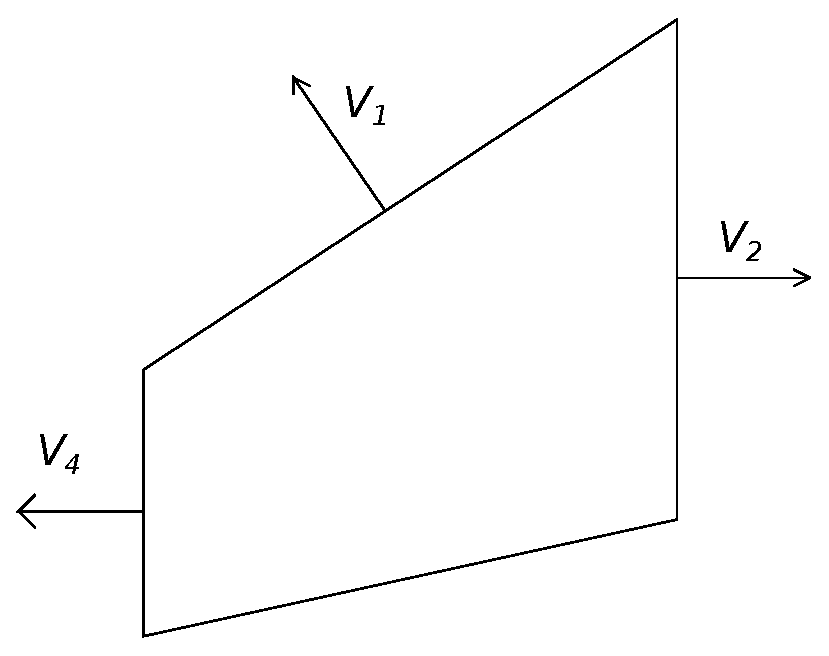
\includegraphics[width=0.5\textwidth]{fig/calculatingFlux.eps}
	\end{figure}
	}
\end{frame}

\begin{frame}
	\frametitle{Numerical Solutions of the Shallow Water Equation}
	\begin{block}{The System of Equations}
		\begin{align*}
		\begin{array}{c c}
		V_t + (u+\sqrt{\eta})V_x = 0, & V = u + 2 \sqrt \eta\\
		U_t + (u-\sqrt{\eta})U_x = 0, & U = u - 2\sqrt \eta
		\end{array}
		\end{align*}
	\end{block}
\end{frame}
\begin{frame}
	\frametitle{Numerical Scheme}
	\only<1-1>{
	\begin{figure}[b]
		\centering
		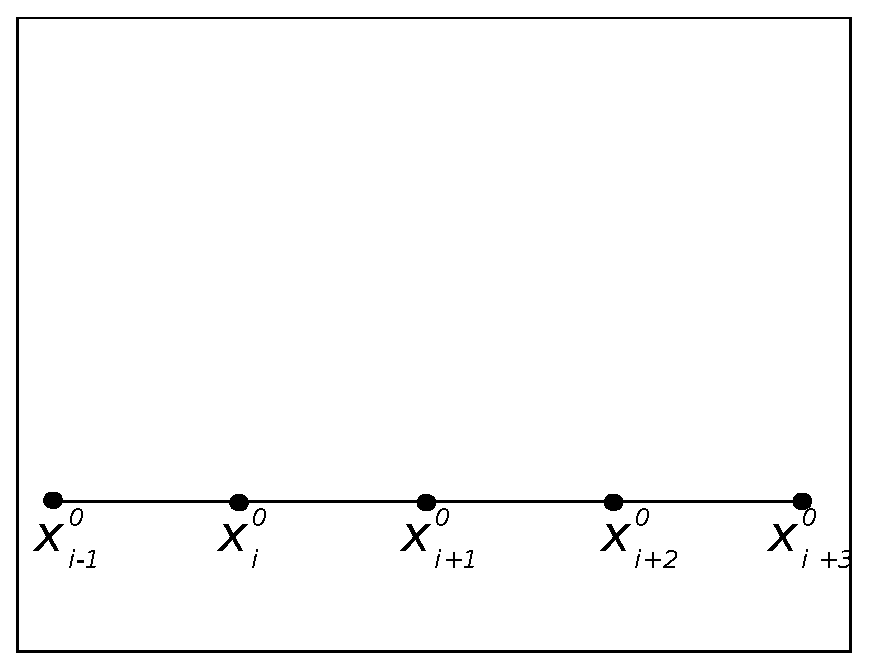
\includegraphics[width=0.7\textwidth]{fig/charWaveEq1stStep.eps}
	\end{figure}
	}
	\only<2-2>{
		\begin{figure}[b]
			\centering
			\includegraphics[width=0.7\textwidth]{fig/charWaveEq2ndStep.eps}
		\end{figure}
	}
	\only<3-3>{
		\begin{figure}[b]
			\centering
			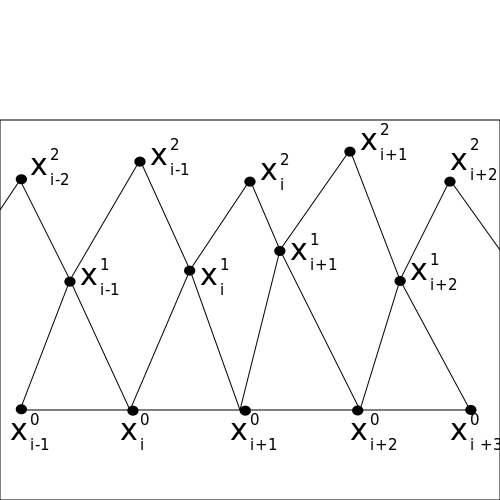
\includegraphics[width=0.7\textwidth]{fig/charWaveEq3rdStep.eps}
		\end{figure}
	}
\end{frame}


\begin{frame}
	\frametitle{Conclusion}
	\begin{itemize}
		\item Time: 3.5 to 4 minutes 
		\item Wave Height: Around $20m$
	\end{itemize}	
\end{frame}



\end{document}